\documentclass {article}

\usepackage[utf8]{inputenc}
\usepackage[english,greek]{babel}
\usepackage{alphabeta}
\usepackage[T1,LGR]{fontenc}

% For more math mode styles
\usepackage{amsmath}

% For images
\usepackage{graphicx}

% For more colors
\usepackage{color}

% Drawing diagrams
\usepackage{tikz}

% Octave code highlighting
\usepackage{listings}

% Links
\usepackage{hyperref}

%% Options

% For hyperlinks
\hypersetup{
	colorlinks=true,
	linkcolor=blue,
	filecolor=magenta,      
	urlcolor=cyan,
}

\urlstyle{same}

% Colors
\definecolor{codegreen}{rgb}{0,0.6,0}
\definecolor{codegray}{rgb}{0.5,0.5,0.5}
\definecolor{codepurple}{rgb}{0.58,0,0.82}
\definecolor{backcolour}{rgb}{0.95,0.95,0.92}
 
% Listing Style
\lstdefinestyle{mystyle}{
	backgroundcolor=\color{backcolour},
    commentstyle=\color{codegreen},
    keywordstyle=\color{magenta},
    numberstyle=\tiny\color{codegray},
    stringstyle=\color{codepurple},
    basicstyle=\scriptsize\ttfamily,
    breakatwhitespace=false,         
    breaklines=true,                 
    captionpos=b,                    
    keepspaces=true,                 
    numbers=left,                    
    numbersep=5pt,                  
    showspaces=false,                
    showstringspaces=false,
    showtabs=false,                  
    tabsize=4
}

\lstset{style=mystyle}

%Tikz options
\usetikzlibrary{fadings}
\usetikzlibrary{backgrounds}
\usetikzlibrary{arrows}
\usetikzlibrary{shapes,shapes.geometric,shapes.misc}

% this style is applied by default to any tikzpicture included via \tikzfig
\tikzstyle{tikzfig}=[baseline=-0.25em,scale=0.5]

% these are dummy properties used by TikZiT, but ignored by LaTex
\pgfkeys{/tikz/tikzit fill/.initial=0}
\pgfkeys{/tikz/tikzit draw/.initial=0}
\pgfkeys{/tikz/tikzit shape/.initial=0}
\pgfkeys{/tikz/tikzit category/.initial=0}

% standard layers used in .tikz files
\pgfdeclarelayer{edgelayer}
\pgfdeclarelayer{nodelayer}
\pgfsetlayers{background,edgelayer,nodelayer,main}

% style for blank nodes
\tikzstyle{none}=[inner sep=0mm]

% Images folder
\graphicspath{{./images/}{./tikz_images/}}

% Paragraph options 
\setlength{\parskip}{\baselineskip}%
\setlength{\parindent}{0pt}%

% Writing in English command
\newcommand{\english}[1]{\foreignlanguage{english}{#1}}

\title{2\textsuperscript{ή} Εργαστηριακή Άσκηση στο μάθημα
Συστήματα Αναμονής}

\author{Λεωνίδας Αβδελάς $|$ AM: 03113182} 

\date{}

\begin{document}

\pagenumbering{gobble}

\maketitle

\pagenumbering{arabic}

\section*{Θεωρητική μελέτη της ουράς Μ/Μ/1}	

\textbf{(α)} Για να είναι η ουρά Μ/Μ/1 εργοδική θα πρέπει να ισχύει η παρακάτω συνθήκη:

\begin{equation} \label{eq:1}
    ρ = \frac{λ}{μ} < 1
\end{equation}

Αν δεν ισχύει η συνθήκη αυτή, η ουρά θα εκραγεί.

Το διάγραμμα ρυθμού μεταβάσεων της ουράς Μ/Μ/1 φαίνεται παρακάτω:   

\tikzset{every picture/.style={line width=0.75pt}} %set default line width to 0.75pt        

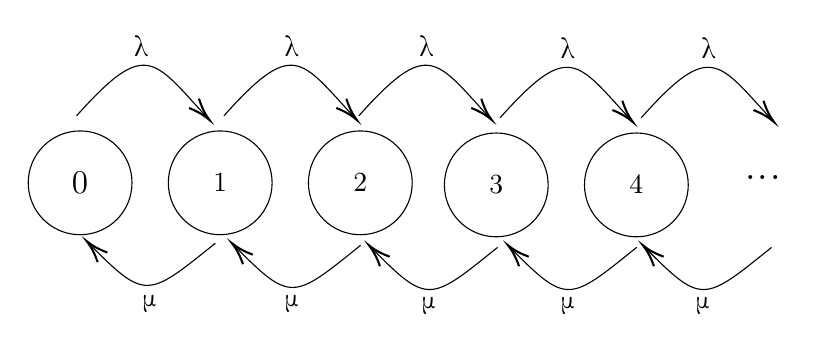
\begin{tikzpicture}[x=0.75pt,y=0.75pt,yscale=-1,xscale=1]
%uncomment if require: \path (0,300); %set diagram left start at 0, and has height of 300

%Shape: Circle [id:dp36463805740392874] 
\draw   (100,137.5) .. controls (100,123.69) and (111.19,112.5) .. (125,112.5) .. controls (138.81,112.5) and (150,123.69) .. (150,137.5) .. controls (150,151.31) and (138.81,162.5) .. (125,162.5) .. controls (111.19,162.5) and (100,151.31) .. (100,137.5) -- cycle ;
%Shape: Circle [id:dp49355021812463695] 
\draw   (167.5,137.5) .. controls (167.5,123.69) and (178.69,112.5) .. (192.5,112.5) .. controls (206.31,112.5) and (217.5,123.69) .. (217.5,137.5) .. controls (217.5,151.31) and (206.31,162.5) .. (192.5,162.5) .. controls (178.69,162.5) and (167.5,151.31) .. (167.5,137.5) -- cycle ;
%Shape: Circle [id:dp871080570996956] 
\draw   (235,137.5) .. controls (235,123.69) and (246.19,112.5) .. (260,112.5) .. controls (273.81,112.5) and (285,123.69) .. (285,137.5) .. controls (285,151.31) and (273.81,162.5) .. (260,162.5) .. controls (246.19,162.5) and (235,151.31) .. (235,137.5) -- cycle ;
%Curve Lines [id:da7742544383995771] 
\draw    (123.3,105.2) .. controls (156.79,67.77) and (160.2,77.88) .. (186.1,105.91) ;
\draw [shift={(187.3,107.2)}, rotate = 227.05] [color={rgb, 255:red, 0; green, 0; blue, 0 }  ][line width=0.75]    (10.93,-3.29) .. controls (6.95,-1.4) and (3.31,-0.3) .. (0,0) .. controls (3.31,0.3) and (6.95,1.4) .. (10.93,3.29)   ;

%Curve Lines [id:da6930765525247415] 
\draw    (194.3,105.2) .. controls (227.79,67.77) and (231.2,77.88) .. (257.1,105.91) ;
\draw [shift={(258.3,107.2)}, rotate = 227.05] [color={rgb, 255:red, 0; green, 0; blue, 0 }  ][line width=0.75]    (10.93,-3.29) .. controls (6.95,-1.4) and (3.31,-0.3) .. (0,0) .. controls (3.31,0.3) and (6.95,1.4) .. (10.93,3.29)   ;

%Curve Lines [id:da03048531539389132] 
\draw    (190.15,166.6) .. controls (157.64,192.7) and (156.67,194.55) .. (129.41,166.88) ;
\draw [shift={(128.15,165.6)}, rotate = 405.5] [color={rgb, 255:red, 0; green, 0; blue, 0 }  ][line width=0.75]    (10.93,-3.29) .. controls (6.95,-1.4) and (3.31,-0.3) .. (0,0) .. controls (3.31,0.3) and (6.95,1.4) .. (10.93,3.29)   ;

%Curve Lines [id:da9416009679387978] 
\draw    (260.15,167.6) .. controls (227.64,193.7) and (226.67,195.55) .. (199.41,167.88) ;
\draw [shift={(198.15,166.6)}, rotate = 405.5] [color={rgb, 255:red, 0; green, 0; blue, 0 }  ][line width=0.75]    (10.93,-3.29) .. controls (6.95,-1.4) and (3.31,-0.3) .. (0,0) .. controls (3.31,0.3) and (6.95,1.4) .. (10.93,3.29)   ;

%Shape: Circle [id:dp08427723786330943] 
\draw   (300.5,138.5) .. controls (300.5,124.69) and (311.69,113.5) .. (325.5,113.5) .. controls (339.31,113.5) and (350.5,124.69) .. (350.5,138.5) .. controls (350.5,152.31) and (339.31,163.5) .. (325.5,163.5) .. controls (311.69,163.5) and (300.5,152.31) .. (300.5,138.5) -- cycle ;
%Shape: Circle [id:dp42950270474251284] 
\draw   (368,138.5) .. controls (368,124.69) and (379.19,113.5) .. (393,113.5) .. controls (406.81,113.5) and (418,124.69) .. (418,138.5) .. controls (418,152.31) and (406.81,163.5) .. (393,163.5) .. controls (379.19,163.5) and (368,152.31) .. (368,138.5) -- cycle ;
%Curve Lines [id:da9218061657658421] 
\draw    (327.3,106.2) .. controls (360.79,68.77) and (364.2,78.88) .. (390.1,106.91) ;
\draw [shift={(391.3,108.2)}, rotate = 227.05] [color={rgb, 255:red, 0; green, 0; blue, 0 }  ][line width=0.75]    (10.93,-3.29) .. controls (6.95,-1.4) and (3.31,-0.3) .. (0,0) .. controls (3.31,0.3) and (6.95,1.4) .. (10.93,3.29)   ;

%Curve Lines [id:da20656772838494564] 
\draw    (393.15,168.6) .. controls (360.64,194.7) and (359.67,196.55) .. (332.41,168.88) ;
\draw [shift={(331.15,167.6)}, rotate = 405.5] [color={rgb, 255:red, 0; green, 0; blue, 0 }  ][line width=0.75]    (10.93,-3.29) .. controls (6.95,-1.4) and (3.31,-0.3) .. (0,0) .. controls (3.31,0.3) and (6.95,1.4) .. (10.93,3.29)   ;

%Curve Lines [id:da3328589967405482] 
\draw    (259.3,105.2) .. controls (292.79,67.77) and (296.2,77.88) .. (322.1,105.91) ;
\draw [shift={(323.3,107.2)}, rotate = 227.05] [color={rgb, 255:red, 0; green, 0; blue, 0 }  ][line width=0.75]    (10.93,-3.29) .. controls (6.95,-1.4) and (3.31,-0.3) .. (0,0) .. controls (3.31,0.3) and (6.95,1.4) .. (10.93,3.29)   ;

%Curve Lines [id:da26545555327288484] 
\draw    (326.15,168.6) .. controls (293.64,194.7) and (292.67,196.55) .. (265.41,168.88) ;
\draw [shift={(264.15,167.6)}, rotate = 405.5] [color={rgb, 255:red, 0; green, 0; blue, 0 }  ][line width=0.75]    (10.93,-3.29) .. controls (6.95,-1.4) and (3.31,-0.3) .. (0,0) .. controls (3.31,0.3) and (6.95,1.4) .. (10.93,3.29)   ;

%Curve Lines [id:da36843765031599873] 
\draw    (395.3,106.2) .. controls (428.79,68.77) and (432.2,78.88) .. (458.1,106.91) ;
\draw [shift={(459.3,108.2)}, rotate = 227.05] [color={rgb, 255:red, 0; green, 0; blue, 0 }  ][line width=0.75]    (10.93,-3.29) .. controls (6.95,-1.4) and (3.31,-0.3) .. (0,0) .. controls (3.31,0.3) and (6.95,1.4) .. (10.93,3.29)   ;

%Curve Lines [id:da5179463443718875] 
\draw    (458.15,168.6) .. controls (425.64,194.7) and (424.67,196.55) .. (397.41,168.88) ;
\draw [shift={(396.15,167.6)}, rotate = 405.5] [color={rgb, 255:red, 0; green, 0; blue, 0 }  ][line width=0.75]    (10.93,-3.29) .. controls (6.95,-1.4) and (3.31,-0.3) .. (0,0) .. controls (3.31,0.3) and (6.95,1.4) .. (10.93,3.29)   ;


% Text Node
\draw (125,137.5) node  [align=left] {{\large 0}};
% Text Node
\draw (260,137.5) node  [align=left] {2};
% Text Node
\draw (192.5,137.5) node  [align=left] {1};
% Text Node
\draw (154.5,71.75) node [scale=0.9] [align=left] {{\selectfont {\large λ}}};
% Text Node
\draw (227,71.75) node [scale=0.9] [align=left] {{\selectfont {\large λ}}};
% Text Node
\draw (158.5,195.95) node  [align=left] {{\selectfont {\small μ}}};
% Text Node
\draw (227,195.95) node  [align=left] {{\selectfont {\small μ}}};
% Text Node
\draw (393,138.5) node  [align=left] {4};
% Text Node
\draw (325.5,138.5) node  [align=left] {3};
% Text Node
\draw (360,72.75) node [scale=0.9] [align=left] {{\selectfont {\large λ}}};
% Text Node
\draw (360,196.95) node  [align=left] {{\selectfont {\small μ}}};
% Text Node
\draw (292,71.75) node [scale=0.9] [align=left] {{\selectfont {\large λ}}};
% Text Node
\draw (293,196.95) node  [align=left] {{\selectfont {\small μ}}};
% Text Node
\draw (428,72.75) node [scale=0.9] [align=left] {{\selectfont {\large λ}}};
% Text Node
\draw (425,196.95) node  [align=left] {{\selectfont {\small μ}}};
% Text Node
\draw (454,135) node  [align=left] {{\LARGE ...}};


\end{tikzpicture}
 

Οι εξισώσεις ισορροπίας της ουράς είναι:

\begin{align} 
	(λ + μ) & p_n = μp_{n+1} + λp_{n-1} \; (n \geq 1), \label{eq:2}\\
	λ & p_{0} = μp_{1} \label{eq:3}
\end{align} 

Χρησιμοποιώντας την εξίσωση \ref{eq:1} και την εξίσωση \ref{eq:3}, έχουμε ότι:

\begin{equation} \label{eq:4}
	p_1 = ρp_0
\end{equation}

Ομοίως, χρησιμοποιώντας την εξίσωση \ref{eq:2} και την εξίσωση \ref{eq:4}, με $n = 1$, έχουμε:

\begin{align*}
	(λ + μ) p_1 & = μp_2 + λp_0 \\
	p_2 & = \frac{(λ+μ) ρ}{μ} p_0 - \frac{λ}{μ}p_0 \\
	p_2 & = ρ^2p_0 + ρp_0 - ρp_0 \\
	p_2 & = ρ^2 p_0
\end{align*}

Χρησιμοποιώντας την σχέση \ref{eq:2} αναδρομικά καταλήγουμε στο αποτέλεσμα:

\begin{equation}\label{eq:5}
	p_n = ρ^np_0 
\end{equation}

Για να υπολογίσουμε το $p_0$, θα χρησιμοποιήσουμε το γεγονός ότι ο τύπος ολικής πιθανότητας για όλες τις πιθανότητες μας λέει ότι το άθροισμα όλων των πιθανοτήτων πρέπει να είναι ίσο με 1, δηλαδή:

\begin{equation}\label{eq:6}
	\sum_{n=0}^{\infty}{p_n} = 1
\end{equation}

Από την εξίσωση \ref{eq:5} και την εξίσωση \ref{eq:6}, θα έχουμε ότι:

\begin{equation}\label{eq:7}
	1 = \sum_{n=0}^{\infty}{p_n} = \sum_{n=0}^{\infty}{ρ^np_0} = p_0\sum_{n=0}^{\infty}{ρ^n}
\end{equation}

Αρα $p_0 = \frac{1}{\sum_{n=0}^{\infty}{ρ^n}}$. Η $\sum_{n=0}^{\infty}{ρ^n}$ είναι γεωμετρική σειρά και αφού $ρ < 1$, η σειρά συγκλίνει σε:

\begin{equation}
	\sum_{n=0}^{\infty}{ρ^n} = \frac{1}{1 - ρ} \; (ρ < 1)
\end{equation}

Τελικά καταλήγουμε στο αποτέλεσμα $p_0 = 1-ρ$.

Άρα οι εργοδικές πιθανότητες του συστήματος είναι:

\begin{align}
	p_n = ρ^n(1-ρ) \label{eq:8} \\
	p_0 = 1-ρ	\label{eq:9}
\end{align}


\textbf{(β)} Για να υπολογίσουμε την μέση κατάσταση του συστήματος σε ισορροπία, θα χρησιμοποιήσουμε την εξίσωση της μέσης τιμής που μας είναι γνωστή από τις πιθανότητες $ E(X) = \sum_{i=1}^k{x_ip_i}$, καθώς και την εξίσωση \ref{eq:8}.

Έτσι έχουμε:

\begin{equation} \label{eq:10}
	\begin{split}
		E[n(t)] = \sum_{n=0}^{\infty}{np_n} \\
		= (1-ρ) \sum_{n=0}^{\infty}{nρ^n}
	\end{split}
\end{equation}

Για  το άθροισμα $\sum_{n=0}^{\infty}{nρ^n}$ έχουμε:

\begin{equation} \label{eq:11}
	\begin{split}
		\sum_{n=0}^{\infty}{nρ^n} & = ρ + 2ρ^2 + 3ρ^3 + ...\\
		& = ρ(1 + 2ρ + 3ρ^2 + ...) \\
		& = ρ \sum_{n=1}^{\infty}{n ρ^{n-1}}
	\end{split}
\end{equation}

Παρατηρούμε ότι $\sum_{n=1}^{\infty}{n ρ^{n-1}}$ είναι η παράγωγος του $\sum_{n=1}^{\infty}{ρ^n}$ ως προς το $ρ$. 

Γνωρίζουμε ότι η γεωμετρική σειρά $\sum_{n=0}^{\infty}{ρ^n}$ ισούται με $\frac{1}{1-ρ}$. Καθώς το άθροισμα μας ξεκινάει από $n = 1$, θα αφαιρέσουμε τον πρώτο όρο από τα δύο μέρη.

\begin{equation} \label{eq:12}
	\begin{split}
		\sum_{n=0}^{\infty}{ρ^n} = \sum_{n=1}^{\infty}{ρ^n} + 1 = \frac{1}{1-ρ}\\
	\Rightarrow \sum_{n=1}^{\infty}{ρ^n} = \frac{1}{1-ρ} - 1 = \frac{ρ}{1-ρ}
	\end{split}
\end{equation}

Άρα από τις εξισώσεις \ref{eq:11} και \ref{eq:12}, έχουμε 

\begin{equation} \label{eq:13}
	\sum_{n=1}^{\infty}{nρ^{n-1}} = \frac{d}{dρ}(\frac{ρ}{1-ρ}) = \frac{1-ρ+ρ}{(1-ρ)^2} = \frac{1}{(1-ρ)^2} 
\end{equation}

Συνδιάζοντας τις εξισώσεις \ref{eq:10}, \ref{eq:11} και \ref{eq:13}, έχουμε:

\begin{equation}
	\begin{split}
		L = E[n(t)] = \frac{ρ(1-ρ)}{(1-ρ)^2} = \frac{ρ}{1-ρ}
	\end{split}	
\end{equation}

Για να βρούμε τον μέσο χρόνο καθυστέρησης, θα χρησιμοποιήσουμε τον Νόμο του \foreignlanguage{english}{Little}, ο οποίος μας λέει ότι o μέσος χρόνος στο σύστημα ανα πελάτη $W$, είναι ανάλογος με τον μέσο αριθμό πελατών $L = E[n(t)]$ που μόλις υπολογίσαμε και τον ρυθμό αφίξεων $λ$, σύμφωνα με την σχέση $W = \frac{L}{λ}$.

Σύμφωνα με τα παραπάνω έχουμε:

\begin{equation}
	W = \frac{L}{λ} = \frac{ρ}{λ(1-ρ)} = \frac{λ / μ}{λ(1-ρ)} = \frac{1 / μ}{1-ρ}
\end{equation}

\textbf{(γ)} Η πιθανότητα το σύστημα μας να βρεθεί με 57 πελάτες είναι $p_{57} = (1-ρ)ρ^{57}$. Δωσμένου του γεγονότος ότι $ρ < 1$, η πιθανότητα αυτή είναι πολύ μικρή, κοντά στο 0. Δεν μπορούμε να απαντήσουμε με βεβαιότητα αν θα υπάρξει τέτοια στιγμή ή όχι.

\textbf{(δ)} Λόγω του γεγονότος ότι οι εξισώσεις ισορροπίας δεν αλλάζουν, δεν θα αλλάξει τίποτα στην ουρά μας αν αρχικά έχει 5 πελάτες αντί για 0. Όλες οι εξισώσεις θα παραμείνουν ίδιες. Αυτό συμβαίνει γιατί μελετάμε το σύστημα όταν είναι σε ισορροπία και όχι στην αρχική ασταθή κατάσταση.

\section*{Ανάλυση ουράς Μ/Μ/1 με \foreignlanguage{english}{Octave}}

\textbf{(α)} Όπως αναφέραμε και στην θεωρητική ανάλυση, οι αποδεκτοί ρυθμοί εξυπηρέτησης θα είναι αυτοί που θα εξασφαλίζουν $ρ = \frac{λ}{μ} < 1$. Αφού $λ = 5$ πελάτες/\foreignlanguage{english}{min}, θα πρέπει $μ > 5$.

\textbf{(β)} Παρακάτω φαίνονται τα ζητούμενα διαγράμματα. Αυτά είναι τα Σχήματα \ref{fig:util}, \ref{fig:delay}, \ref{fig:requests} και \ref{fig:throughput}.

\begin{figure}[ht]
	\includegraphics[width=\linewidth]{M-M-1_Util_SrvRate}
	\caption{Βαθμός χρησιμοποίησης \foreignlanguage{english}{(utilization)} προς ρυθμό εξυπηρέτησης (μ).}
	\label{fig:util}
\end{figure}

\begin{figure}[ht]
	\includegraphics[width=\linewidth]{M-M-1_AvgDlay_SrvRate}
	\caption{Μέσος χρόνος καθυστέρησης του συστήματος $E(T)$ προς ρυθμό εξυπηρέτησης (μ).}
	\label{fig:delay}
\end{figure}

\begin{figure}[ht]
	\includegraphics[width=\linewidth]{M-M-1_AvgRqsts_SrvRate}
	\caption{Μέσος αριθμός πελατών στο σύστημα προς ρυθμό εξυπηρέτησης (μ).}
	\label{fig:requests}
\end{figure}

\begin{figure}[ht]
	\includegraphics[width=\linewidth]{M-M-1_Thrpt_SrvRate}
	\caption{Ρυθμαπόδοση (\foreignlanguage{english}{Throughput}) πελατών προς ρυθμό εξυπηρέτησης (μ).}
	\label{fig:throughput}
\end{figure}

\textbf{(γ)} Όπως βλέπουμε όσο αυξάνεται ο μέσος ρυθμός εξυπηρέτησης, τόσο μειώνεται και ο μέσος χρόνος καθυστέρησης. Όμως, για τιμές μεγαλύτερες από $μ=7$, ο ρυθμός με τον οποίο μειώνεται ο μέσος χρόνος καθυστέρησης είναι πολύ μικρός. Άρα, μια τιμή γύρω στο $μ = 7$ μας εξασφαλίζει πολύ καλά αποτελέσματα με χαμηλότερο κόστος. 

\textbf{(δ)} Παρατηρούμε ότι το \foreignlanguage{english}{throughput} είναι σταθερό και ίσο με $λ$. Αυτό εξηγήται, γιατί η ρυθμαπόδοση ορίζεται ως $μ\sum_{j=1}^{\infty}{π_j}$, δηλαδή ο ρυθμός που επεξεργάζεται κάθε κατάσταση το σύστημα. Από την παραπάνω σχέση έχουμε:

\begin{equation}
	μ\sum_{j=1}^{\infty}{π_j} = μ(1-π_0) = μρ = λ
\end{equation}

\section*{Σύγκριση συστημάτων με δύο εξυπηρετητές}

Μας δίνεται σύστημα αναμονής με μέσο ρυθμό αφίξεων $λ = 10$ πελάτες/\foreignlanguage{english}{min}.
Θα συγρίνουμε μια ουρά Μ/Μ/2 με εκθετικούς εξυπηρετητές μέσου ρυθμού εξυπηρέτησης $μ = 10$ πελάτες/\foreignlanguage{english}{min} ανα εξυπηρετητή και δύο παράλληλες ουρές Μ/Μ/1 με εκθετικό χρόνο εξυπηρέτησης $μ = 10$ πελάτες/\foreignlanguage{english}{min} η καθεμία.

Σαν μέτρο σύγρκισης θα χρησιμοποιήσουμε το μέσο χρόνο καθυστέρησης.

Για την ουρά Μ/Μ/2 με τα παραπάνω χαρακτηριστικά έχουμε ότι ο μέσος χρόνος καθυστέρησης είναι $0.133$ \foreignlanguage{english}{min}.

Για τις δύο παράλληλες ουρές, καθώς είναι ισοπίθανο και τυχαίο το σε ποιά ουρά θα πάει ο κάθε νέος πελάτης, μπορούμε να θεωρήσουμε ότι κάθε σύστημα Μ/Μ/1 έχει μέσο ρυθμό αφίξεων κατανομή \foreignlanguage{english}{Poisson} με $λ_i = 5,\;i = 1, 2$ πελάτες/\foreignlanguage{english}{min}. Ο συνολικός ρυθμός αφίξεων παραμένει $λ = \sum_{i=1}^{2}{λ_i} = 10$ πελάτες/\english{min}.

O μέσος ρυθμός χρόνος καθυστέρησης θα είναι ο μέσος όρος των δύο ουρών.

Σύμφωνα με τα παραπάνω καταλήγουμε ότι ο μέσος χρόνος καθυστέρησης για τις δύο Μ/Μ/1 ουρές είναι $0.2$ \english{min}.

Σύμφωνα με τα στοιχεία αυτά θα επιλέγαμε την ουρά Μ/Μ/2, γιατί ο χρόνος αναμονής είναι μικρότερος. Αυτό εξηγήται από το γεγονός ότι στην ουρά Μ/Μ/2, όταν υπάρχει πελάτης στην ουρά, θα εξυπηρετηθεί μόλις απελευθερωθεί κάποιος από τους εξυπηρετητές. Στην περίπτωση των Μ/Μ/1 ουρών, οι πελάτες κατανέμονται τυχαία, που συμαίνει ότι η μια ουρά είναι άδεια, αλλά στην άλλη περιμένουν παραπάνω από ένας πελάτες, γεγονός που αυξάνει την μέση καθυστέρηση.

\section*{Διαδικασία γεννήσεων θανάτων \\
(\english{birth-death process}): εφαρμογή\\
σε σύστημα Μ/Μ/1/Κ}

\textbf{(α)} Για το σύστημα έχουμε ότι $λ_0 = λ$, $λ_1 = \frac{λ}{2}$, $λ_2 = \frac{λ}{3}$ και $λ_3 = \frac{λ}{4}$ (για $i \geq 4, λ_i = 0$), ενώ $μ_i = μ,\; i = 0, 1, 2, 3, 4$. Αρα το σύστημα έχει 5 καταστάσεις. Το διάγραμμα ρυθμού μεταβάσεων φαίνεται παρακάτω:

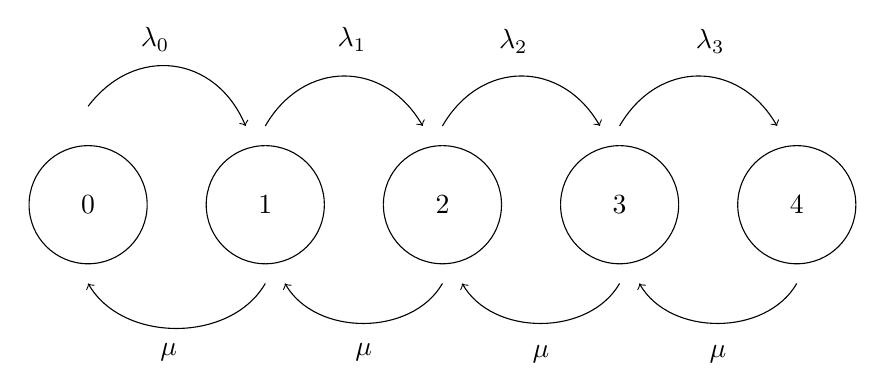
\begin{tikzpicture}
	\tikzstyle{arrow}=[->]
	\begin{pgfonlayer}{nodelayer}
		\node [style=none] (0) at (0, 0.75) {};
		\node [style=none] (2) at (0, -0.75) {};
		\node [style=none] (3) at (0.75, 0) {};
		\node [style=none] (4) at (-0.75, 0) {};
		\node [style=none] (5) at (2.25, 0.75) {};
		\node [style=none] (6) at (2.25, -0.75) {};
		\node [style=none] (7) at (3, 0) {};
		\node [style=none] (8) at (1.5, 0) {};
		\node [style=none] (9) at (4.5, 0.75) {};
		\node [style=none] (10) at (4.5, -0.75) {};
		\node [style=none] (11) at (5.25, 0) {};
		\node [style=none] (12) at (3.75, 0) {};
		\node [style=none] (13) at (6.75, 0.75) {};
		\node [style=none] (14) at (6.75, -0.75) {};
		\node [style=none] (15) at (7.5, 0) {};
		\node [style=none] (16) at (6, 0) {};
		\node [style=none] (17) at (0, 1.25) {};
		\node [style=none] (18) at (2, 1) {};
		\node [style=none] (19) at (2.25, 1) {};
		\node [style=none] (20) at (4.25, 1) {};
		\node [style=none] (21) at (4.5, 1) {};
		\node [style=none] (22) at (6.5, 1) {};
		\node [style=none] (23) at (0, -1) {};
		\node [style=none] (24) at (2.25, -1) {};
		\node [style=none] (25) at (2.5, -1) {};
		\node [style=none] (26) at (4.5, -1) {};
		\node [style=none] (27) at (4.75, -1) {};
		\node [style=none] (28) at (6.75, -1) {};
		\node [style=none] (29) at (0, 0) {$0$};
		\node [style=none] (30) at (2.25, 0) {$1$};
		\node [style=none] (31) at (4.5, 0) {$2$};
		\node [style=none] (32) at (6.75, 0) {$3$};
		\node [style=none] (33) at (0.85, 2.1) {$λ_0$};
		\node [style=none] (34) at (3.35, 2.1) {$λ_1$};
		\node [style=none] (36) at (5.4, 2.075) {$λ_2$};
		\node [style=none] (37) at (5.75, -1.9) {$μ$};
		\node [style=none] (38) at (3.5, -1.875) {$μ$};
		\node [style=none] (39) at (1.025, -1.875) {$μ$};
		\node [style=none] (40) at (9, 0.75) {};
		\node [style=none] (41) at (9, -0.75) {};
		\node [style=none] (42) at (9.75, 0) {};
		\node [style=none] (43) at (8.25, 0) {};
		\node [style=none] (44) at (6.75, 1) {};
		\node [style=none] (45) at (8.75, 1) {};
		\node [style=none] (46) at (7, -1) {};
		\node [style=none] (47) at (9, -1) {};
		\node [style=none] (48) at (9, 0) {$4$};
		\node [style=none] (49) at (7.9, 2.075) {$λ_3$};
		\node [style=none] (50) at (8, -1.9) {$μ$};
	\end{pgfonlayer}
	\begin{pgfonlayer}{edgelayer}
		\draw [bend left=45] (0.center) to (3.center);
		\draw [bend left=45] (3.center) to (2.center);
		\draw [bend right=45] (0.center) to (4.center);
		\draw [bend right=45] (4.center) to (2.center);
		\draw [bend left=45] (5.center) to (7.center);
		\draw [bend left=45] (7.center) to (6.center);
		\draw [bend right=45] (5.center) to (8.center);
		\draw [bend right=45] (8.center) to (6.center);
		\draw [bend left=45] (9.center) to (11.center);
		\draw [bend left=45] (11.center) to (10.center);
		\draw [bend right=45] (9.center) to (12.center);
		\draw [bend right=45] (12.center) to (10.center);
		\draw [bend left=45] (13.center) to (15.center);
		\draw [bend left=45] (15.center) to (14.center);
		\draw [bend right=45] (13.center) to (16.center);
		\draw [bend right=45] (16.center) to (14.center);
		\draw [style=arrow, bend left=60, looseness=1.25] (17.center) to (18.center);
		\draw [style=arrow, bend left=60, looseness=1.25] (19.center) to (20.center);
		\draw [style=arrow, bend left=60, looseness=1.25] (21.center) to (22.center);
		\draw [style=arrow, bend left=60] (24.center) to (23.center);
		\draw [style=arrow, bend left=60] (26.center) to (25.center);
		\draw [style=arrow, bend left=60] (28.center) to (27.center);
		\draw [bend left=45] (40.center) to (42.center);
		\draw [bend left=45] (42.center) to (41.center);
		\draw [bend right=45] (40.center) to (43.center);
		\draw [bend right=45] (43.center) to (41.center);
		\draw [style=arrow, bend left=60, looseness=1.25] (44.center) to (45.center);
		\draw [style=arrow, bend left=60] (47.center) to (46.center);
	\end{pgfonlayer}
\end{tikzpicture}


Από τις εξισώσεις ισορροπίας έχουμε: 

\begin{equation}\label{eq:14}
	\begin{split}
		λ_0p_0 & = μ_1p_1\\
		(λ_n + μ_n)p_n & = λ_{n-1}p_{n-1} + μ_{n+1}p_{n+1},\; n \geq 1
	\end{split}
\end{equation}

Από τις εξισώσεις \ref{eq:14} έχουμε ότι:

\begin{equation}\label{eq:15}
	\begin{split}
		p_1 & = \frac{λ_0p_0}{μ_1}\\
		p_{n+1} & = \frac{(λ_n + μ_n)p_n - λ_{n-1}p_{n-1}}{μ_{n+1}},\; n \geq 1
	\end{split}
\end{equation}

Χρησιμοποιώντας αναδρομικά τον τύπο \ref{eq:15}, καταλήγουμε στο παρακάτω αποτέλεσμα:

\begin{equation}\label{eq:16}
	p_n = p_0 \prod_{i=1}^{n}{\frac{λ_{i-1}}{μ_i}},\; n \geq 1
\end{equation}

Θέλουμε να υπολογίσουμε τις εργοδικές ικανότητες από την εξίσωση \ref{eq:16}. Αρχικά θα πρέπει να υπολογίσουμε το $p_0$. Για να το κάνουμε αυτό θα χρησιμοποιήσουμε το γεγονός ότι το άθροισμα όλων των πιθανοτήτων πρέπει να ισούται με 1. Άρα:

\begin{equation}
	\begin{split}		
	p_0 & = \left(1 + \sum_{n=1}^{4}{\prod_{i=1}^{n}{\frac{λ_{i-1}}{μ_i}}} \right)^{-1} \Rightarrow\\
	p_0 & = \left(1 + \prod_{i=1}^{1}{\frac{λ_{i-1}}{μ_i}} 
	+ \prod_{i=1}^{2}{\frac{λ_{i-1}}{μ_i}} \prod_{i=1}^{3}{\frac{λ_{i-1}}{μ_i}} + \prod_{i=1}^{4}{\frac{λ_{i-1}}{μ_i}}\right)^{-1} \Rightarrow\\
	p_0 & = \left(1 + \frac{λ_0}{μ_1} + \frac{λ_0 λ_1}{μ_1 μ_2} +
	 \frac{λ_0 λ_1 λ_2}{μ_1 μ_2 μ_3}  + \frac{λ_0 λ_1 λ_2 λ_3}{μ_1 μ_2 μ_3 μ_4} \right)^{-1} \label{eq:17}
\end{split}
\end{equation}

Γνωρίζοντας ότι $λ = 5$ και $μ = 10$, αρα $λ_0 = 5$, $λ_1 = \frac{5}{2}$, $λ_2 = \frac{5}{3}$, $λ_3 = \frac{5}{4}$ και $ μ_i = 10,\; i = 1, 2, 3$. Αρα απο την εξίσωση \ref{eq:17} και τα παραπάνω, έχουμε τελικά:

\begin{equation}
	\begin{split}
		p_0 & = \left(1 + \frac{5}{10} + \frac{5 \frac{5}{2}}{10^2} +
			 \frac{5 \frac{5}{2} \frac{5}{3}}{10^3} +
			 \frac{5 \frac{5}{2} \frac{5}{3} \frac{5}{4}}{10^4}\right)^{-1} \\
		p_0 & = \left(1 + 0.5 + \frac{25}{200} + \frac{125}{6000} + 
		\frac{625}{240000}\right)^{-1}\\
		p_0 & = 0.607 \label{eq:18}
	\end{split}
\end{equation}

Αφού βρήκαμε το $p_0$, τώρα μπορούμε εύκολα να βρούμε τις υπόλοιπες πιθανότητες. Έτσι, έχουμε: 
\begin{equation}
	\begin{split}
		p_1 & = \frac{λ_0}{μ_1}p_0 = 0.5 \cdot 0.61 = 0.303\\
		p_2 & = \frac{λ_1}{μ_2}p_1 = \frac{\frac{5}{2}}{10} \cdot 0.305 = 0.076\\
		p_3 & = \frac{λ_2}{μ_3}p_2 = \frac{\frac{5}{3}}{10} \cdot 0.076 = 0.0126\\
		p_4 & = \frac{λ_3}{μ_4}p_3 = \frac{\frac{5}{4}}{10} \cdot 0.0126 = 0.0016 
 	\end{split}
\end{equation}

Η πιθανότητα απώλειας πελάτη είναι η πιθανότητα $p_4$, άρα είναι $0.0016$.

\textbf{(β)} \textbf{\english{i.}} Με την βοήθεια του \english{Octave}, έχουμε το παρακάτω πίνακα μεταβάσεων χρησιμοποιώντας την εντολή \english{\lstinline[language=Matlab]{ctmcbd}}:

\begin{equation*}
	\begin{pmatrix} 
		-5 &     5 &       0 &     0 &    0\\
		10 & -12.5 &     2.5 &     0 &    0\\
		0 &     10 & -11.67 &   1.67 &    0\\
		0 &      0 &     10 & -11.25 & 1.25\\
		0 &      0 &      0 &     10 &  -10
	\end{pmatrix}
\end{equation*}

\textbf{\english{ii.}} Χρησιμοποιώντας την εντολή \english{\lstinline[language=Matlab]{ctmc}}, έχουμε τις πιθανότητες:
\begin{equation}
	\begin{split}
		p_0 & = 0.6066351\\
		p_1 & = 0.3033175\\
		p_2 & = 0.0758294\\
		p_3 & = 0.0126382\\
		p_4 & = 0.0015798
	\end{split}
\end{equation}

\begin{figure}
	\includegraphics[width=\linewidth]{ergodic_probabilities}
	\caption{Εργοδικές πιθανότητες συστήματος Μ/Μ/1/4.}
	\label{fig:probs}
\end{figure}

Όπως βλέπουμε, τα αποτελέσματα αυτά επιβεβαιώνουν τα θεωρητικά αποτελέσματα που βρήκαμε στο ερώτημα \textbf{(α)} (Τα αποτελέσματα στο ερώτημα \textbf{(α)} είχαν στρογγυλοποιηθεί για ευκολία των πράξεων). Στο σχήμα \ref{fig:probs} φαίνεται και το \english{bar chart} των πιθανοτήτων για κάθε κατάσταση.

\english{\textbf{iii.}} Ο μέσος όρος των πελατών στο σύστημα βρίσκεται από την μέση τιμή των εργοδικών πιθανοτήτων, δηλαδή:

\begin{equation}
	E(T) = \sum_{i=1}^{4}{i p_i} = 0.5
\end{equation}

\english{\textbf{iv.}} Όπως αναφέρθηκε ήδη, η πιθανότητα απόρριψης πελάτη \english{blocking probability} από το σύστημα είναι η πιθανότητα της κατάστασης 4, δηλαδή $p_4 = 0.0015798$.

\english{\textbf{v.}} Γνωρίζουμε ότι το σύστημα ξεκινάει χωρίς πελάτες, αρα θα ξεκινήσει από την κατάσταση 0. Έτσι υπολογίζουμε τις μεταβατικές περιόδους για κάθε κατάσταση στα Σχήματα \ref{fig:trans_0}, \ref{fig:trans_1}, \ref{fig:trans_2}, \ref{fig:trans_3} και \ref{fig:trans_4}:

\begin{figure}
	\includegraphics[width=\linewidth]{trans_0}
	\caption{Μεταβατική περίοδος για την κατάσταση 0.}
	\label{fig:trans_0}
\end{figure}

\begin{figure}
	\includegraphics[width=\linewidth]{trans_1}
	\caption{Μεταβατική περίοδος για την κατάσταση 1.}
	\label{fig:trans_1}
\end{figure}

\begin{figure}
	\includegraphics[width=\linewidth]{trans_2}
	\caption{Μεταβατική περίοδος για την κατάσταση 2.}
	\label{fig:trans_2}
\end{figure}

\begin{figure}
	\includegraphics[width=\linewidth]{trans_3}
	\caption{Μεταβατική περίοδος για την κατάσταση 3.}
	\label{fig:trans_3}
\end{figure}

\begin{figure}
	\includegraphics[width=\linewidth]{trans_4}
	\caption{Μεταβατική περίοδος για την κατάσταση 4.}
	\label{fig:trans_4}
\end{figure}

\textbf{\english{vi.}} Σε αυτό το βήμα επαναλάβαμε το βήμα \textbf{\english{v.}} για διάφορες τιμές του $μ$. Έτσι για $μ = 1$ έχουμε το σχήμα \ref{fig:trans_mu_1}, για $μ = 5$ έχουμε το σχήμα \ref{fig:trans__mu_5} και για $μ = 20$ έχουμε το σχήμα \ref{fig:trans_mu_20}.

\begin{figure}
	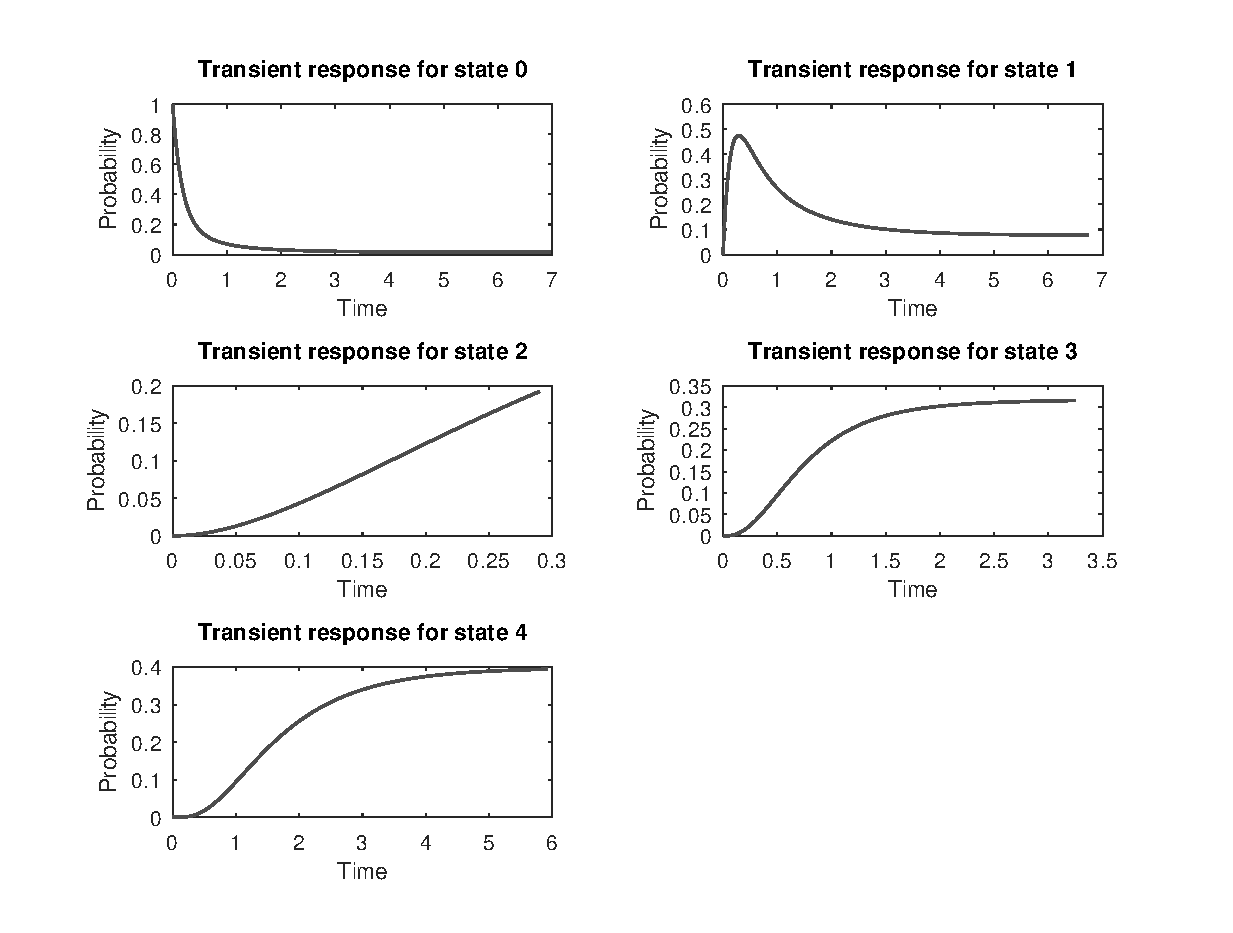
\includegraphics[width=\linewidth]{trans_mu_1}
	\caption{Μεταβατική περίοδος όλων των καταστάσεων για $μ = 1$.}
	\label{fig:trans_mu_1}
\end{figure}

\begin{figure}
	\includegraphics[width=\linewidth]{trans_mu_5}
	\caption{Μεταβατική περίοδος όλων των καταστάσεων για $μ = 5$.}
	\label{fig:trans__mu_5}
\end{figure}

\begin{figure}
	\includegraphics[width=\linewidth]{trans_mu_20}
	\caption{Μεταβατική περίοδος όλων των καταστάσεων για $μ = 20$.}
	\label{fig:trans_mu_20}
\end{figure}

Όπως αναμέναμε, βλέπουμε ότι όσο το $μ$ μικραίνει, η πιθανότητα των μικρότερων καταστάσεων στην σταθερή κατάσταση είναι μικρότερη, δηλαδή το σύστημα να έχει στην ουρά λίγους πελάτες και η πιθανότητα των μεγαλύτερων καταστάσεων (3 και 4) είναι αρκετά μεγάλη. Ακόμα για μικρό $μ$, η σταθερότητα σε όλες τις καταστάσεις έρχεται πολύ αργά σε σχέση με μεγάλα $μ$.

\section*{Παράρτημα: Κώδικας \english{Octave}}

\selectlanguage{english}
\lstinputlisting[language=Octave]{Assignment2.m}

\end{document}